\documentclass{beamer}
\usepackage{owl}
\usepackage{tikz}
\usetikzlibrary{shapes}
\usetheme{default}
\begin{document}

\begin{frame}{Background}
We say two justifications $\J_{1}$ and $\J_{2}$ are \emph{isomorphic} if there exists a \emph{bijective} function $\phi$ that maps entity names in $\J_{1}$ to entity names in $\J_{2}$. Example:
\begin{align*}
\J_{1} &= \{ A \sqsubseteq B \sqcap \exists r.C, B \sqcap \exists r.C \sqsubseteq D\} \models A \sqsubseteq D\\
\J_{2} &= \{ E \sqsubseteq B \sqcap \exists s.F, B \sqcap \exists s.F  \sqsubseteq D\} \models E \sqsubseteq D
\end{align*}

In this example, the mapping $\phi$ maps $A$ to $E$, $r$ to $s$, $C$ to $F$, and all others names to themselves. 

Things we know about this relation:
\begin{itemize}
\item $\phi$ is bijective (condition).
\item Strict isomorphism is reflexive (easy to see: $\phi = id$), symmetric (because $\phi$ is a bijection), and transitive (why?).
\end{itemize}

\end{frame}

\begin{frame}{Subexpression-Isomorphism}
We can extend this strict isomorphism to allow mappings between \emph{subexpressions} as in the following example: 
\begin{align*}
\J_{1} &= \{A \sqsubseteq B \sqcap C, B \sqcap C \sqsubseteq D \} \models A \sqsubseteq D  \\ 
\J_{2} &= \{ A \sqsubseteq \exists r.C, \exists r.C  \sqsubseteq D\} \models A \sqsubseteq D
\end{align*}

For this purpose we introduce a \emph{template} $(\theta, \eta)$ and two mapping functions $\phi_1$ and $\phi_2$.

\begin{definition} Two justifications $(\J_{1}, \eta_1)$ and $(\J_{2}, \eta_2)$ are \emph{s-isomorphic} if there exists a template $(\theta, \eta)$ and two mapping functions $\phi_1$ and $\phi_2$ such that $\phi_{1}(\theta, \eta) = (\J_{1}, \eta_{1})$ and $\phi_{2}(\theta) = (\J_{2},\eta_2)$.
\end{definition}
\end{frame}

\begin{frame}{The Problem}
We want to prove that s-isomorphism is \emph{transitive}. We know that
\begin{itemize}
\item $\phi_1$ and $\phi_2$ are \emph{not} surjective in the strict sense: the number of subexpressions  in $(\J_{1}, \eta_1)$ and $(\J_{2}, \eta_2)$ can be larger than the number of names in $(\theta, \eta)$ due to nesting. Surjectivity can be achieved by requiring the ranges of the mappings to be signature disjoint (i.e. something like $\phi_{1}  = \{x \mapsto B, y \mapsto \exists r.B \}$ is not a legal mapping). If we enforce signature-disjointness, subex-iso is ``downwards-compatible'' with strict iso.
\item s-iso is reflexive (for $(\theta, \eta) = (\J_1, \eta_1), \phi_1 = id, \phi_2 = id$).
\item s-iso is symmetric (I find it obvious - but why?)
\end{itemize}

\end{frame}

\begin{frame}{Proof: Goal}
Given:
\begin{itemize}
\item 3 justifications $(\J_{a}, \eta_{a}), (\J_{b}, \eta_{b}) , (\J_{c}, \eta_{c}) $
\item Assume
\begin{itemize}
\item $(\J_{a}, \eta_{a}) \sisom (\J_{b}, \eta_{b}) $ via $\phi^{ab}_{1}, \phi^{ab}_{2}, (\Theta_{ab}, \eta_{ab})$
\item $(\J_{b}, \eta_{b}) \sisom (\J_{c}, \eta_{c}) $ via $\phi^{bc}_{1}, \phi^{bc}_{2}, (\Theta_{bc}, \eta_{bc})$
\end{itemize}
\end{itemize}

We want to show that it is always possible to construct a template $(\Theta_{ac}, \eta_{ac})$ and the mappings $\phi^{ac}_{1}, \phi^{ac}_{2}$ such that  $(\J_{a}, \eta_{a}) \sisom (\J_{c}, \eta_{c}) $ via $\phi^{ac}_{1}, \phi^{ac}_{2}, (\Theta_{ac}, \eta_{ac})$.

\end{frame}

\begin{frame}{Proof: The situation}
\begin{figure}
\centering
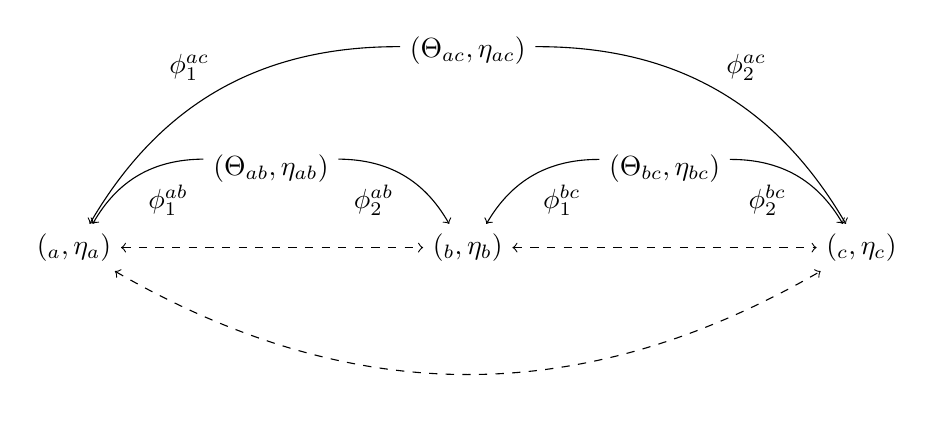
\begin{tikzpicture}
  [scale=1,->,auto=left,every node/.style={draw=none, fill=none}]

  \node (tab) at (3.5,9) {$ (\Theta_{ab}, \eta_{ab})$};
  \node (tbc) at (8.5,9) {$(\Theta_{bc}, \eta_{bc})$};
  \node (tac) at (6,10.5) {$(\Theta_{ac}, \eta_{ac})$};
    
  \node (ja) at (1,8) {$(\J_{a}, \eta_{a})$};
  \node (jb) at (6,8) {$(\J_{b}, \eta_{b}) $};
  \node (jc) at (11,8) {$(\J_{c}, \eta_{c}) $};

  \draw [bend right] (tab) to node {$\phi^{ab}_{1}$} (ja);
  \draw [bend left] (tab) to node [swap] {$\phi^{ab}_{2}$} (jb);
  \draw [ bend right] (tbc) to node {$\phi^{bc}_{1}$} (jb);
  \draw [bend left] (tbc) to node [swap]  {$\phi^{bc}_{2}$} (jc);
  
  \draw [bend right] (tac) to node [swap]  {$\phi^{ac}_{1}$} (ja);
  \draw [bend left] (tac) to node {$\phi^{ac}_{2}$} (jc);


  \draw [<->, dashed] (ja) to node {$\sisom$} (jb);
  \draw [<->, dashed] (jb) to node [swap] {$\sisom$} (jc);
  \draw [<->, dashed, bend right] (ja) to node {$\sisom$} (jc);
    
\end{tikzpicture}
\end{figure}

\end{frame}

\begin{frame}{Example: Construction of $(\Theta_{ac}, \eta_{ac})$}

\centering
\scalebox{0.7}{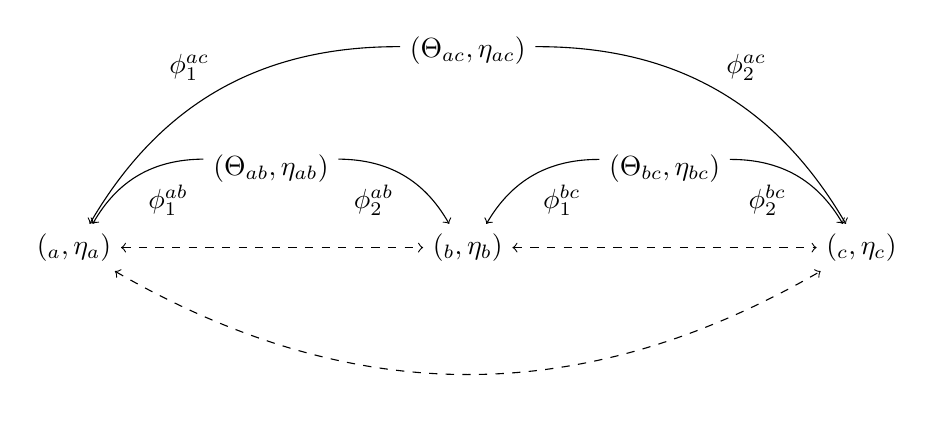
\begin{tikzpicture}
  [scale=1,->,auto=left,every node/.style={draw=none, fill=none}]

  \node (tab) at (3.5,9) {$ (\Theta_{ab}, \eta_{ab})$};
  \node (tbc) at (8.5,9) {$(\Theta_{bc}, \eta_{bc})$};
  \node (tac) at (6,10.5) {$(\Theta_{ac}, \eta_{ac})$};
    
  \node (ja) at (1,8) {$(\J_{a}, \eta_{a})$};
  \node (jb) at (6,8) {$(\J_{b}, \eta_{b}) $};
  \node (jc) at (11,8) {$(\J_{c}, \eta_{c}) $};

  \draw [bend right] (tab) to node {$\phi^{ab}_{1}$} (ja);
  \draw [bend left] (tab) to node [swap] {$\phi^{ab}_{2}$} (jb);
  \draw [ bend right] (tbc) to node {$\phi^{bc}_{1}$} (jb);
  \draw [bend left] (tbc) to node [swap]  {$\phi^{bc}_{2}$} (jc);
  
  \draw [bend right] (tac) to node [swap]  {$\phi^{ac}_{1}$} (ja);
  \draw [bend left] (tac) to node {$\phi^{ac}_{2}$} (jc);


  \draw [<->, dashed] (ja) to node {$\sisom$} (jb);
  \draw [<->, dashed] (jb) to node [swap] {$\sisom$} (jc);
  \draw [<->, dashed, bend right] (ja) to node {$\sisom$} (jc);
    
\end{tikzpicture}}
\begin{align*}
\J_{a} &= \{A1 \sqsubseteq A2 \sqcap A4, A2 \sqcap A4 \sqsubseteq A3 \} \models A1 \sqsubseteq A3  \\ 
\J_{b} &= \{ B1 \sqsubseteq \exists r.B2, \exists r.B2 \sqsubseteq B3\} \models B1 \sqsubseteq B3 \\
\J_{c} &= \{ C1 \sqsubseteq C2, C2  \sqsubseteq C3 \} \models C1 \sqsubseteq C3 \\
\theta_{ab} &= \{ x \sqsubseteq y, y  \sqsubseteq z\} \models x \sqsubseteq z \\
\theta_{bc} &= \{ x' \sqsubseteq y', y'  \sqsubseteq \} \models x' \sqsubseteq z'
\end{align*}

\end{frame}



\begin{frame}{Proof: Construction of $(\Theta_{ac}, \eta_{ac})$}

\centering
\scalebox{0.5}{%
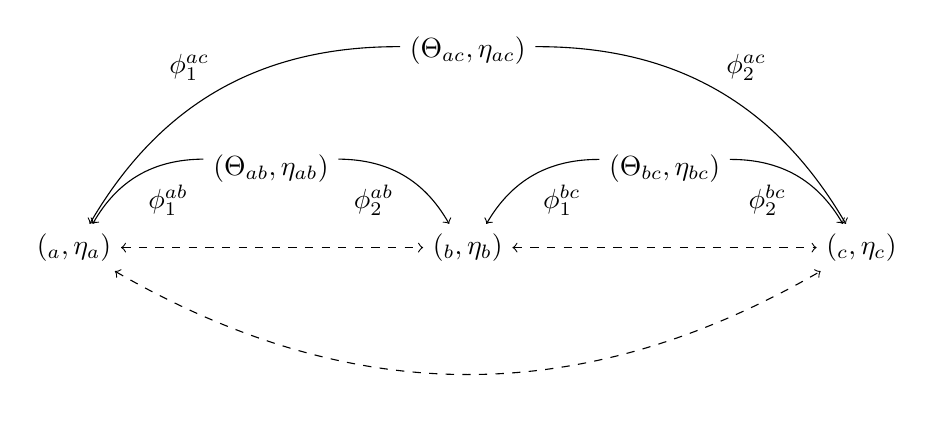
\begin{tikzpicture}
  [scale=1,->,auto=left,every node/.style={draw=none, fill=none}]

  \node (tab) at (3.5,9) {$ (\Theta_{ab}, \eta_{ab})$};
  \node (tbc) at (8.5,9) {$(\Theta_{bc}, \eta_{bc})$};
  \node (tac) at (6,10.5) {$(\Theta_{ac}, \eta_{ac})$};
    
  \node (ja) at (1,8) {$(\J_{a}, \eta_{a})$};
  \node (jb) at (6,8) {$(\J_{b}, \eta_{b}) $};
  \node (jc) at (11,8) {$(\J_{c}, \eta_{c}) $};

  \draw [bend right] (tab) to node {$\phi^{ab}_{1}$} (ja);
  \draw [bend left] (tab) to node [swap] {$\phi^{ab}_{2}$} (jb);
  \draw [ bend right] (tbc) to node {$\phi^{bc}_{1}$} (jb);
  \draw [bend left] (tbc) to node [swap]  {$\phi^{bc}_{2}$} (jc);
  
  \draw [bend right] (tac) to node [swap]  {$\phi^{ac}_{1}$} (ja);
  \draw [bend left] (tac) to node {$\phi^{ac}_{2}$} (jc);


  \draw [<->, dashed] (ja) to node {$\sisom$} (jb);
  \draw [<->, dashed] (jb) to node [swap] {$\sisom$} (jc);
  \draw [<->, dashed, bend right] (ja) to node {$\sisom$} (jc);
    
\end{tikzpicture}
}

\begin{itemize}
\item Goal: We want to construct $(\theta_{ac}, \eta_{ac})$ as a combination of $(\theta_{ab}, \eta_{ab})$ and $(\theta_{bc}, \eta_{bc})$.
\item Take $\J_{b}, \eta_{b}$ and parse into their parse trees. 
\item $\J_{b}|_{p}$ denotes the subtree of $\J_{b}$ at position $p$.
\item $\J_{b}[s \rightarrow t]$ is the tree obtained by replacing, in $\J_{b}$, the subtree at position $s$ with $t$.
\item Label each position $p$ in their parse trees with variables:
\begin{itemize}
\item $(x, ab)$ if $\phi^{ab}_{2}(x) = \J_{b}|_{p}$ and $\Theta_{ab}|_{p} = x$
\item $(x, bc)$ if $\phi^{bc}_{1}(x) = \J_{b}|_{p}$ and $\Theta_{bc}|_{p} = x$
\end{itemize}
\end{itemize}


\end{frame}

\begin{frame}{Example: Construction of $(\Theta_{ac}, \eta_{ac})$}

We obtain the following labelled parse trees:
\begin{itemize}
\item root
\begin{itemize}
\item \subcls
\begin{itemize}
\item (x,ab)
\item (y,ab)
\end{itemize}
\item \subcls
\begin{itemize}
\item (y,ab)
\item (y,bc)
\end{itemize}
\end{itemize}
\end{itemize}

\begin{itemize}
\item \subcls
\begin{itemize}
\item (x,ab)
\item (z,ab)
\end{itemize}
\end{itemize}

Note: (x, ab), (y, ab) and (z, ab) could just as well be (x', bc), (y', bc), and (z', bc) or labelled with both in this case since both conditions hold.

\end{frame}

\begin{frame}{Example: Construction of $(\Theta_{ac}, \eta_{ac})$}

We can then construct $(\Theta_{ac}, \eta_{ac})$ from the parse trees:
\begin{itemize}
\item Remove all subtrees below the labelled nodes.
\item Turn each labelled node (x, ab) or (x,bc) into a leaf node labelled with x.
\item Parse the resulting trees into justification and entailment.
\end{itemize}

In our example, this results in the template $(\Theta_{ac}, \eta_{ac}) = ( \{ x \subcls y, y \subcls z \}, x \subcls z)$.
\end{frame}


\begin{frame}{Construction of $\phi^{ac}_{1}$ and $\phi^{ac}_{2}$}

\begin{figure}
\centering{
\scalebox{0.5}{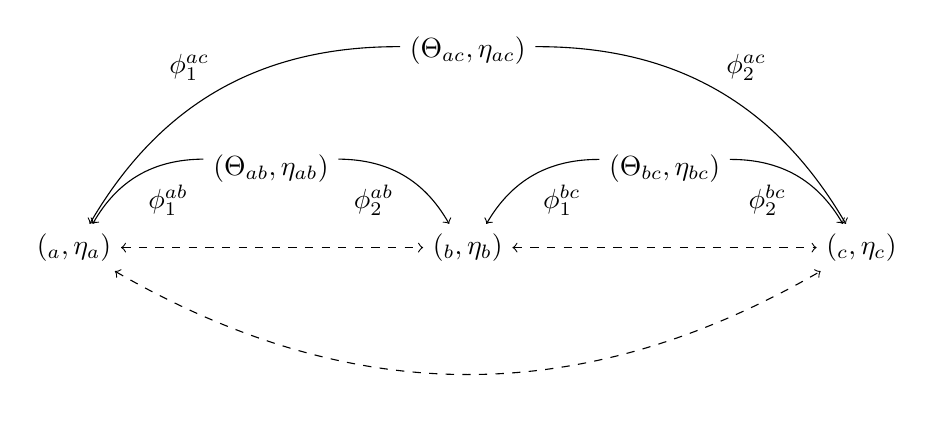
\begin{tikzpicture}
  [scale=1,->,auto=left,every node/.style={draw=none, fill=none}]

  \node (tab) at (3.5,9) {$ (\Theta_{ab}, \eta_{ab})$};
  \node (tbc) at (8.5,9) {$(\Theta_{bc}, \eta_{bc})$};
  \node (tac) at (6,10.5) {$(\Theta_{ac}, \eta_{ac})$};
    
  \node (ja) at (1,8) {$(\J_{a}, \eta_{a})$};
  \node (jb) at (6,8) {$(\J_{b}, \eta_{b}) $};
  \node (jc) at (11,8) {$(\J_{c}, \eta_{c}) $};

  \draw [bend right] (tab) to node {$\phi^{ab}_{1}$} (ja);
  \draw [bend left] (tab) to node [swap] {$\phi^{ab}_{2}$} (jb);
  \draw [ bend right] (tbc) to node {$\phi^{bc}_{1}$} (jb);
  \draw [bend left] (tbc) to node [swap]  {$\phi^{bc}_{2}$} (jc);
  
  \draw [bend right] (tac) to node [swap]  {$\phi^{ac}_{1}$} (ja);
  \draw [bend left] (tac) to node {$\phi^{ac}_{2}$} (jc);


  \draw [<->, dashed] (ja) to node {$\sisom$} (jb);
  \draw [<->, dashed] (jb) to node [swap] {$\sisom$} (jc);
  \draw [<->, dashed, bend right] (ja) to node {$\sisom$} (jc);
    
\end{tikzpicture}}
}
\end{figure}

Now we need to construct the mappings  $\phi^{ac}_{1}$ and $\phi^{ac}_{2}$--again, as a combination of the existing mappings. We do this based on the labelled parse tree and template we just generated:

\begin{itemize}
\item Take the template $(\Theta_{ac}, \eta_{ac})$ and the labelled parse trees.
\item $\phi^{ac}_{1}(x) = \phi^{ab}_{2}(x)$ if a variable x in the template originates from a label (x,ab) in the parse tree of $(\J_{b}, \eta_{b})$ (analogue holds for variables originating from a label (x, bc)).
\item for all positions $s_{j}$ in $\J_{b}$ that are labelled with $(y_{j}, bc)$, $\phi^{ac}_{2}$ is $\J_{b} [s_{j} \rightarrow \phi^{bc}_{2}(y_{j})]$. That is, $\phi^{ac}_{2}(x)$ corresponds to the range variable in $\phi^{bc}_{2}$.
\end{itemize}

\end{frame}


\begin{frame}{Example: Construction of $\phi^{ac}_{1}$ and $\phi^{ac}_{2}$}

\begin{figure}
\centering{
\scalebox{0.5}{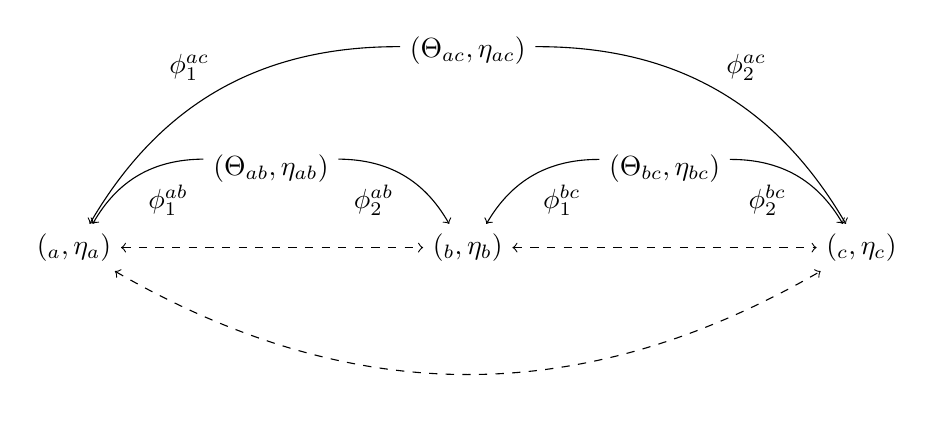
\begin{tikzpicture}
  [scale=1,->,auto=left,every node/.style={draw=none, fill=none}]

  \node (tab) at (3.5,9) {$ (\Theta_{ab}, \eta_{ab})$};
  \node (tbc) at (8.5,9) {$(\Theta_{bc}, \eta_{bc})$};
  \node (tac) at (6,10.5) {$(\Theta_{ac}, \eta_{ac})$};
    
  \node (ja) at (1,8) {$(\J_{a}, \eta_{a})$};
  \node (jb) at (6,8) {$(\J_{b}, \eta_{b}) $};
  \node (jc) at (11,8) {$(\J_{c}, \eta_{c}) $};

  \draw [bend right] (tab) to node {$\phi^{ab}_{1}$} (ja);
  \draw [bend left] (tab) to node [swap] {$\phi^{ab}_{2}$} (jb);
  \draw [ bend right] (tbc) to node {$\phi^{bc}_{1}$} (jb);
  \draw [bend left] (tbc) to node [swap]  {$\phi^{bc}_{2}$} (jc);
  
  \draw [bend right] (tac) to node [swap]  {$\phi^{ac}_{1}$} (ja);
  \draw [bend left] (tac) to node {$\phi^{ac}_{2}$} (jc);


  \draw [<->, dashed] (ja) to node {$\sisom$} (jb);
  \draw [<->, dashed] (jb) to node [swap] {$\sisom$} (jc);
  \draw [<->, dashed, bend right] (ja) to node {$\sisom$} (jc);
    
\end{tikzpicture}}
}
\end{figure}

The resulting mappings for our example are:

\begin{itemize}
\item $\phi^{ac}_{1} = \{ x \mapsto B1, y \mapsto \exists r.B2, z \mapsto B3 \}$ (straightforward because all variables in  $\Theta_{ac}$ originate from (x, ab) type labels.)
\item $\phi^{ac}_{2} = \{ x \mapsto C1, y \mapsto C2, z \mapsto C3 \}$ (straightforward in this case as well)
\end{itemize}

\end{frame}


\begin{frame}{Proof: Entailment of $(\Theta_{ac}, \eta_{ac})$}
\begin{figure}
\centering{
\scalebox{0.5}{%
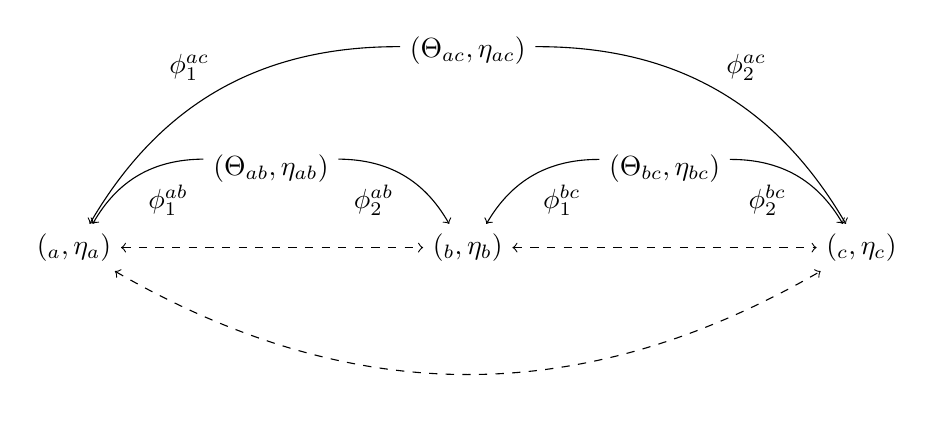
\begin{tikzpicture}
  [scale=1,->,auto=left,every node/.style={draw=none, fill=none}]

  \node (tab) at (3.5,9) {$ (\Theta_{ab}, \eta_{ab})$};
  \node (tbc) at (8.5,9) {$(\Theta_{bc}, \eta_{bc})$};
  \node (tac) at (6,10.5) {$(\Theta_{ac}, \eta_{ac})$};
    
  \node (ja) at (1,8) {$(\J_{a}, \eta_{a})$};
  \node (jb) at (6,8) {$(\J_{b}, \eta_{b}) $};
  \node (jc) at (11,8) {$(\J_{c}, \eta_{c}) $};

  \draw [bend right] (tab) to node {$\phi^{ab}_{1}$} (ja);
  \draw [bend left] (tab) to node [swap] {$\phi^{ab}_{2}$} (jb);
  \draw [ bend right] (tbc) to node {$\phi^{bc}_{1}$} (jb);
  \draw [bend left] (tbc) to node [swap]  {$\phi^{bc}_{2}$} (jc);
  
  \draw [bend right] (tac) to node [swap]  {$\phi^{ac}_{1}$} (ja);
  \draw [bend left] (tac) to node {$\phi^{ac}_{2}$} (jc);


  \draw [<->, dashed] (ja) to node {$\sisom$} (jb);
  \draw [<->, dashed] (jb) to node [swap] {$\sisom$} (jc);
  \draw [<->, dashed, bend right] (ja) to node {$\sisom$} (jc);
    
\end{tikzpicture}
}}
\end{figure}
Now that we have constructed $(\Theta_{ac}, \eta_{ac})$ and the mappings $\phi^{ac}_{1}, \phi^{ac}_{2}$, we need to show that $\Theta_{ac}$ does in fact entail $\eta_{ac}$. Some ideas:

\begin{itemize}
\item Show that $\phi^{ac}_{1}(\Theta_{ac}) = \J_{a}$ and $\phi^{ac}_{1}(\eta_{ac}) =  \eta_{a})$ and likewise for $\phi^{ac}_{2}$ and $(\J_{c}, \eta_{c})$.
\item Show that every model of $\Theta_{ac}$ is a model for $\eta_{ac}$.
\item \ldots?
\end{itemize}

\end{frame}

\end{document}